%\documentclass[11pt,draftclsnofoot,onecolumn,journal,letterpaper]{IEEEtran}
\documentclass{IEEEtran}

\usepackage[UTF8]{ctex}
\usepackage{graphicx}
\begin{document}

\title{基于强化学习的无线网络自组织性研究}
%\author{沈聪,王超,王芷阳}
\maketitle

\begin{abstract}
为了全面的了解无线自组织网络(SON)的智能化发展现状,本文以强化学习算法在SON的技术方面的进展为重点,对现有的相关文献进行综合型研究。文章全面展示了自组织技术应用于蜂窝网络的现有文献,并对实现SON具体功能时涉及到的强化学习(RL)算法和技术展开一系列对比研究。文章的工作主要是为读者提供对实现SON相关功能的最新算法的理解和分类。文章将SON 的相关应用分为自配置、自优化、自愈合三大模块,每个模块包含若干种具体实例。此外本文还从算法的可扩展性,复杂度,鲁棒性,收敛性等多重参数标准,对文章中涉及的算法的进行综合对比,对实际不同场景中的适用的算法提出一般性准则。最后,文章总结本文所做工作,阐述了强化学习算法应用于未来网络可能遇到的挑战,并对自组织网络未来发展方向提出指导意见。
\end{abstract}

\section{引言}
%从5G的发展引入SON技术,并说明leaning算法的应用趋势
在5G系统中,移动通信面对更加多样化的业务需求和指标,系统采用了更为复杂的无线传输技术和融合的无线网络架构,融合了多种接入方式、多种制式、多种架构的异构网络。超密集组网使得未来网络将进一步使现有的小区结构微型化、分布化 , 并加强小区间的相互协作;LTE、UMTS、WiFi 等多种制式网络将在5G中共存;SDN/NFV等虚拟化架构引入到5G 当中,而更多密集的小型基站甚至支持“即插即用”等更加便捷智能的配置。因此,网络管理复杂度远远高于现有网络,网络深度智能化成为保证 5G 网络性能的迫切需要,使得更加智能的自组织网络(Self Organizing Network, SON)将成为 5G 不可或缺的关键技术。为了全面的了解SON的智能化发展现状,本文以强化学习算法在SON的技术方面的进展为重点,对现有的相关文献进行详细的综合研究。

\subsection{自组织网络简介}

%介绍无线自组织网络发展现状,以及部署在5G网络中的具体应用
%强调learning算法在SON中应用的必要性。

在传统的移动通信网络中,网络部署、运维等基本依靠人工的方式,需要投入大量的人力,给运营商带来巨大的基本建设成本(Capital Expenditure, CAPEX)和运行成本(Operational expenditure,OPEX)。并且,随着移动通信网络的发展,依靠人工的方式难以实现网络的优化。因此,为了解决网络部署、优化的复杂性问题,降低运维成本相对总收入的比例,使运营商能高效运营、维护网络,在满足客户需求的同时,自身也能够持续发展,由下一代移动网络(Next Generation Mobile Network,NGMN)联盟中的运营商主导,联合主要的设备制造商提出了自组织网络的概念\cite{Alliance2008}。由于 5G 将采用大规模 MIMO 无线传输技术,使得空间自由度大幅度增加,从而带来天线选择、协作节点优化、波束选择、波束优化、多用户联合资源调配等方面的灵活性。对这些技术的优化,是5G 系统SON技术的重要内容。自组织网络的思路是在网络中引入自组织能力即实现网络智能化,包括自配置、自优化、自愈合等实现网络规划、部署、维护、优化和排障等各个环节的自动进行,最大限度地减少人工干预,并结合先进的学习理论逐步提升网络智能化。


\subsection{强化学习简介}

%简单概括强化学习定义,泛化介绍其特点,应用,不用展开,第二部分会具体讲
%介绍强化学习的发展现状,与通信场景结合实际应用的可行性分析。

SON在蜂窝网络中被定义为一个网络的概念,不仅具有自适应和自主功能,而且还具有足够的可扩展性,稳定性和灵活性,即使在环境发生变化时也能保持其期望的目标。虽然学习的方法没有直接包含在SON的定义中,但学习算法在系统功能的实现以及自动维护的问题上可以代替人工更有效地解决预料之外的问题。\emph{强化学习(Reinforcement Learning, RL)}是一种应用较为普遍的学习算法,这种算法以环境的状态作为输入,通过系统与环境的交互和试错,根据在交互过程中产生的评价性反馈信号,实现最终决策的不断优化。传统的有监督学习(Supervised Learning)依靠有标签的数据样本通过分类器推断功能,从而得到新实例的映射。无监督学习(Unsupervised Learning)相反是针对无标签数据进行自主结构性学习的过程。强化学习类似无监督学习,同样不需要预先标记的数据,不同的是强化学习依靠与环境及状态的实时信息交互,即从环境中获得回报并依此调整策略,逐渐获得最大化的预期收益。
\begin{figure}%[h]
\centerline{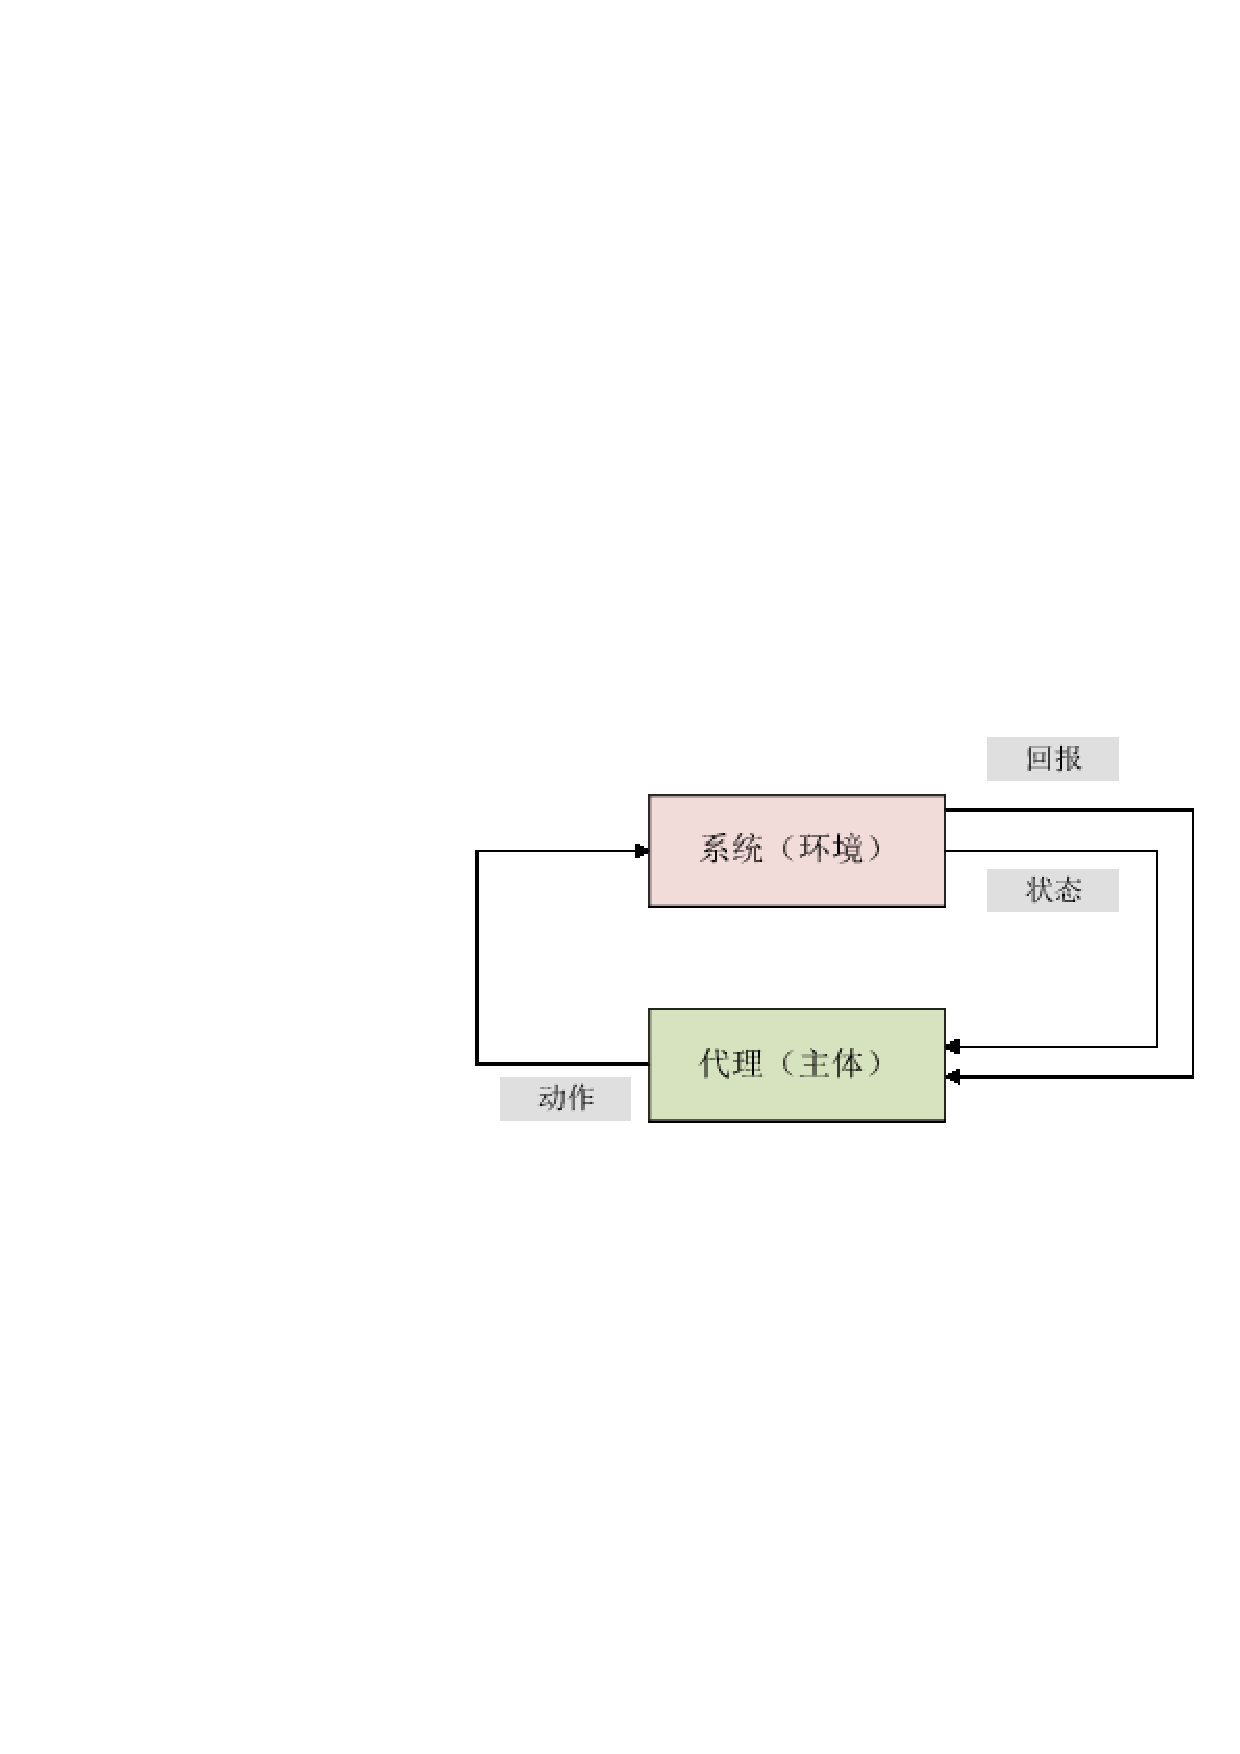
\includegraphics[width=0.4\textwidth]{reinforcement.pdf}}
%\vspace{4em}
\caption{强化学习过程}
\label{fig:rein}
\end{figure}

图\ref{fig:rein}直观说明了强化学习的典型过程:进行学习操作的主体收到系统的状态以及与上一次状态转换相关的回报函数,之后主体依据历史信息计算出下一步的操作传送给系统。作为回应,系统转换到下一状态并不断重复上述过程。整个问题的目的在于逐渐学习一系列操作来控制系统,从而最大化总的回报函数。强化学习中包含几类不同的问题,将在第\ref{sec:RL}部分中具体叙述,区别主要在于系统返回数据的方式以及不同的性能度量方法。


\subsection{本文工作}

如前所述,本文的目标之一是在过去的十年中对在蜂窝网络领域实施智能解决方案进行广泛的文献回顾,以便总结管理日益复杂网络的相关技术。本文不仅介绍了与SON相关的最新研究成果,而且还对现有涉及RL算法实现管理自组织网络的技术进行总结。
本文的主要贡献有以下几个方面:
\begin{itemize}
  \item 文章全面展示了自组织网络技术应用于蜂窝网络的现有文献,并对实现SON具体功能时涉及到的RL算法和技术展开一系列对比研究;
  \item 本文的重点是应用于SON的强化学习算法,文章的工作主要是为读者提供对实现这些SON功能的最新算法的理解和分类,避免了对SON的功能进行过于详细的描述;
  \item 文章将SON的相关应用分为自配置、自优化、自愈合三大模块,每个模块包含若干种实例。对于研究不同实例的参考文献,我们在文章中进行详细的分类研究;
  \item 本文还从算法的可扩展性,复杂度,鲁棒性,收敛性等多重参数标准,对文章中涉及的算法的进行综合对比,对实际不同场景中的适用的算法提出一般性准则;
  \item 最后,文章总结本文所做工作,阐述了RL算法可能遇到的挑战,并对自组织网络未来发展方向提出指导意见。
\end{itemize}

具体内容分为以下几个部分:第\ref{sec:RL}部分介绍强化学习的发展,以及应用较为广泛的算法。第\ref{sec:SON}部分对SON 的发展中出现的问题进行介绍,并分类总结强化学习在各种问题下的应用。第\ref{sec:Compare}部分对比各类算法在解决SON中问题的性能进行分析。第\ref{sec:FutureWork}以及\ref{sec:Conclusion}部分分别展望未来SON发展方向,以及强化学习面临的新型问题,并对本文涉及的相关内容进行总结。
\section{强化学习}
\label{sec:RL}

强化学习是在系统的基础上,通过\emph{代理(Agent)}与周围环境的交互,以获得描述当前\emph{系统状态(State)}的信息量用于选择对于当前环境应当做出的\emph{动作(Action)}。与其他学习算法不同的是,强化学习的系统在执行某个行为之后会反馈给代理一个信息量,\emph{收益(Reward)} 或者\emph{损失(Loss)}, 用于评估此行为的优劣\cite{Sutton1998}。

一般来讲,强化学习的模型分为以下四个部分:
\begin{itemize}
\item \emph{策略(Policy)}:表示代理根据系统当前状态做出的相应的动作;
\item \emph{回报函数(Reward function)}:提供了对当前系统状态的评估,由此前采取的动作确定返回的信息量——收益或者损失;
\item \emph{值函数(Value function)}:代理处维持的一些策略收益性能的评估值,依据此来找到最大化收益的长期策略;
\item \emph{环境模型(Environment model)}:决定系统的状态集合以及代理可能采取的动作集合。
\end{itemize}

由于强化学习算法具有评估每次行为的奖励机制,因此存在\emph{探索(Exploration)}与\emph{利用(Exploitation)}之间的权衡关系,具体表现为代理必须决定在接下来的策略中,究竟是在系统中探索其他动作,以发现未知动作带来的更高收益,还是依据已知信息最大限度地利用当前已知最高收益的动作。

强化学习发展至今,具有广泛应用的模型有以下两种:多摇臂赌博机(Multi-armed Bandit,MAB),有限马尔科夫决策过程(Markov Decision Process,MDP)。两类模型又包含多种具体模型以及算法思想。下面将简单介绍几类模型以及算法,并给出一些常用模型在蜂窝网络通信中的具体应用。

%Q- 学习算法是利用Q- 函数计算并不断优化,以得到系统的最佳策略。基于Q-学习算法,\cite{Kaelbling1996} 中结合模糊逻辑的相关控制方法,形成一套有效的强化学习算法,称为模糊Q-学习算法。对于上述强化学习算法的具体过程将在第\ref{sec:RL} 部分中详细介绍,此外关于具体算法应用于SON 的相关问题,将在接下来的部分分别展开讨论。

\subsection{多摇臂赌博机问题(MAB)}
多摇臂赌博机(MAB)问题的实际原型即为一个玩家在赌场中面对一排(单摇臂)赌博机时,每台机器都有自己赢钱的概率而玩家不知道,玩家需要决定玩哪一台机器,在每台机器上玩几次,按什么顺序玩这些机器来让自己赢尽可能多的钱。将这一排单臂赌博机看作一个多摇臂赌博机,就成为了我们所研究的多摇臂赌博机模型。从理论上来定义,MAB问题是由一系列动作决定的资源序列分配问题。在每个时隙,单位资源被分配给一个动作并获得回馈收益,问题目标是最大化获得的总收益值,基本点是选择当前回馈收益最优的动作与选择未来可能有更大回馈收益动作之间的冲突。由此可以看出回报起到两个作用:一是增加总收益值,二是提供信息以推测各动作的性能表现。MAB问题目前已经在蜂窝网络通信问题中得到了广泛应用,例如Zhang等人在\cite{Zhang2017}中研究基站的能量存储管理与负载控制;Maghsudi等人在\cite{Maghsudi2017}中研究动态小基站网络中用户接入问题;Wang等人在\cite{Wang2017}中研究企业网络中小基站的功率自优化问题等等。MAB问题应用广泛的原因还在于它具有多种变形模型,接下来我们简单介绍几类比较常用的变形模型。
\subsubsection{随机性多摇臂赌博机(Stochastic Bandit)}
在随机性MAB问题中,每个摇臂上的回报都服从一个未知的统计概率分布,相当于每个摇臂的性能是可以确定的。这样解决此类MAB问题的思想在于估计出每个摇臂的性能并尽可能多选择性能最好的摇臂,目前常用的算法有利用频率方法或贝叶斯方法。前一种主要有随机选取非估计最优的$\epsilon$-greedy算法\cite{Sutton2016},以及联合考虑估计值与估计的不确定度的置信区间上界(Upper Confidence Bound UCB)算法       \cite{Auer2002a}。利用贝叶斯思想的主要有汤普森抽样(Thompson Sampling)\cite{Agrawal2012}\cite{Kaufmann2012},以及根据后验分布改进的Bayes-UCB算法\cite{Kaufmann2012a}。基于这些基本的算法思想,可以考虑模型中的变形问题,例如每个摇臂性能随时间变化的不稳定情况,每个摇臂可能在某一段时间内不可用的情况,以及摇臂性能之间具有相关性等多种变形。这些变形的模型在一定情况下与通信场景可以建立非常直接的联系,使得MAB 算法可以用来高效的解决目前高密度网络中面对的问题。

目前有很多已有工作,比如Shen等人在\cite{Shen2017}中利用随机性MAB算法解决小基站切换问题;Simsek等人在\cite{Simsek2015a}中利用UCB算法解决异构网中的干扰控制问题;Wang等人在Wang等人在\cite{Wang2017}中利用摇臂间具有相关性以及贝叶斯思想来自动优化室内小基站的信号发射功率。

\subsubsection{对抗性多摇臂赌博机(Adversarial Bandit)}
对抗性MAB与随机性MAB不同,回到最初对MAB模型直观的说明,对抗性MAB相当于是在一个有作弊手段的赌场里,店家可以操作赌博机,在每个时隙可以任意设定回报来满足自身利益,每次调整回报可能依赖也可能独立于以往的决策动作。在这种情况下,每个摇臂的性能不再能用一个具体的概率分布来描述,即回报是非随机的。在这种问题下,随机性决策算法经常被使用,最基础的EXP3算法\cite{Auer2002}利用指数权重分配的思想计算出每个时隙选择所有摇臂的概率,依此概率进行决策。相应地,在对抗性MAB问题中也存在着不稳定,部分摇臂不可用等相应的变形模型,在相关文献中也有具体的理论分析。

目前主要利用对抗性MAB模型来解决非随机的问题,例如,Maghsudi等人在\cite{Maghsudi2017}中基于EXP3算法解决小基站网络中用户关联问题;Shen等人\cite{Shen2016}中利用改进的分批EXP3算法解决异构网中考虑频繁切换的用户移动性接入问题。

\subsubsection{有情境赌博机(Contextual Bandit)}
MAB的另一种变形模型为对每个摇臂关联辅助信息,这些辅助信息被描述为摇臂的相关情境。在这种模型下,策略需要根据情境选择合适的摇臂。在实际的通信系统中,例如在Simsek等人在\cite{Simsek2015a}中,当用户看作摇臂时,用户的移动速度、数据传输速率等因素就可以看作是相关情境信息,从而利用相关算法有效解决用户与基站的关联问题。



\subsubsection{有状态赌博机(Markovian Bandit)}
在有状态MAB模型中,每个摇臂都与有限状态空间相关联。摇臂被选择之后,返回一个回报之后,摇臂的状态依照一定的模型发生转化,一般为马尔科夫过程。基于这种模型,在 中提出了基于惠特尔指标策略来解决此种MAB模型。Sun等人在\cite{Sun2017}中利用用户行为特征来优化异构网中基站与用户的关联问题,其中用户作为基站,其移动速度等特征可以看作其状态;在\cite{Tekin2011}中,此模型用于解决机会频谱接入问题。

%常见的MAB算法分类,以及我们组所做相关工作。

%\subsection{Q-学习算法}

%重点介绍,Q-学习方法应用较多,基于此方法添加模糊逻辑,形成的模糊Q-学习方法在通信中的应用较为广泛。

\subsection{有限马尔科夫决策过程}
MDP问题是满足马尔科夫性质的一类强化学习问题。一个特定的马尔科夫决策过程由状态、动作集与环境的一步动态定义。由于对状态及策略的具体建模,MDP可以在普遍程度上刻画大部分的强化学习问题。在马尔科夫决策问题中一般依据贝尔曼方程,通过求解最优值函数来获得最优策略。传统的解决方法一般利用动态规划,但对于状态空间较大的情况复杂度较高不易处理。

\subsubsection{Q-学习}
强化学习中较常用的估计值函数的方法为Q-学习算法,利用产生的Q函数估计序列逐渐收敛于最优值,Q-学习方法在强化学习的著作
\cite{Sutton2016}等书中均有详细讲解。在\cite{Simsek2015} 中,作者为解决异构网中基站选择问题,将问题建模为马尔科夫过程:用户可看作代理中心,状态为用户目前所在的基站,此时用户想进行基站切换,动作即为在邻基站列表中选择切换到其他基站从而获得更好的性能。利用现有的Q-学习算法进行迭代运算,可以获得最优策略。在
\cite{Ghadimi2017} 中,作者同样利用马尔科夫模型以及Q-学习算法解决了蜂窝网络中下行链路的功率控制问题。
\cite{Dhahri2012}中,作者运用Q-学习算法解决动态场景下用户在进行切换时的基站选择问题。

\subsubsection{模糊 Q-学习}
考虑到Q-学习方法在状态-动作空间较大时,计算储存Q函数值将耗费大量空间与时间,因此将Q-学习方法扩展到模糊推理系统,可以近似存储Q函数值,并且可以利用先验知识来减少训练量。模糊Q-学习方法需要将输入的状态与动作空间划分为模糊的集合,因此离散化后的Q函数值可以使一部分必要的Q函数值在查找表中计算并存储。根据此设定,\cite{Glorennec1997}等文章对原有Q-学习算法做出了相应改进。在实际的自组织网络中,当强化学习用于解决一系列网络自动化问题时,输入输出空间经常是连续或高维的变量,模糊系统作为有效的解决方法可以与强化学习技术相结合,扩展后的模糊Q-学习方法在网络问题中应用更为广泛。在
\cite{Munoz2013} 中,作者利用模糊Q-学习算法解决企业小基站网络中负载均衡问题。在\cite{Razavi2010}中,作者使用模糊Q-学习方法用来解决LTE 网络中基站覆盖范围的自优化问题。\cite{Fan2014}中,作者利用Q-学习方法训练模糊神经网络中模糊系统中的从属函数参数。Dirani等人在\cite{Dirani2010}中利用模糊Q-学习方法通过调整基站功率分配实现网络中的干扰控制。


\section{自组织网络应用发展}
\label{sec:SON}
%本文的重点章节,各个技术应用的问题介绍清楚,分类所有的强化学习的文章
%LTE的部署对SON的推进,涉及到若干问题及其解决方案。
%下列各种应用对应的实际问题可以参考\cite{Klaine2017}中Introduction部分的分类。
5G将多种制式网络融合为一种协同的异构网络,从技术上来看,网络中存在多层、多种无线接入技术,导致其管理功能的实现比现有网络更为复杂,因而网络的部署、运营、维护需要引入更为智能化的解决方案。5G 将采用超密集的异构网络节点部署方式,意味着网络中在宏基站的覆盖范围内存在大量如微基站等类似的低功率节点\cite{Moysen2017},因此,在网络拓扑、系统间干扰、用户负载均衡处理、基站部署规划、用户设备移动性方面都将表现出与现有无线网络明显不同之处,网络节点的自动配置和维护将成为运营商面临的重要挑战。

因此,在诸多问题及挑战下,未来 5G 网络应该支持更智能的 SON 功能\cite{Imran2014}。首先,在自配置功能方面,由于低功率节点在网络中大量部署,导致基站的邻区关系的复杂度呈指数上升,需要发展面向随机部署、超密集网络场景的新的自动邻区关系技术,以支持网络节点接入即可使用。其次,在自优化方面,网络的密度增加会导致每个基站存在多个不同的干扰源,加上用户移动性、网络运行过程中的随机因素, 使协调技术的优化更为困难。最后,自愈合方面,由于网络中的业务随时间和空间动态变化,引起低功率节点在运行过程中的不确定性,会造成接入点随机开启关闭等故障现象,同样也需要自组织网络功能以实现的智能化补偿。在接下来的部分中,文章将分别从三个方面介绍SON的相关用例以及解决方案。
\subsection{自配置应用}
\label{sec:self-configuration}

在SON中,自配置是指自动配置当前网络中,如微基站,中继站,宏基站等所有设备参数的过程。此外,若当前网络系统已经开始运行,又有新网络节点引入以及设置,或者网络从故障中重新启动,此时自配置包括站点位置选择、硬件配置标准化以及每个新网络节点的准备、安装、鉴权和认证,基本涵盖了将一个新节点纳入网络中运行的全部过程 \cite{Aliu2013}。针对SON中出现的不同类型问题,\cite{Wainio2016}提出了一种通用框架,在自配置的角度,该框架提供实现网络自组织的所需的一些基本步骤,首先在部署之前,基站已经配置基本的操作参数,这些参数对于各种实际应用场景是不变的,因此不需要再次部署。其次,第二阶段的配置包括扫描并确定基站的相邻基站,建立起邻基站列表(Neighbour Cell List,NCL)。最后阶段是基于现有网络拓扑,对新部署的基站后的网络进行参数调整。与该方法不同的是 \cite{Hu2010}文中提出的部署新基站的方式为感知并选中一个相邻基站进行所必须的参数请求以及下载。因此,自配置的基本应用包括以下三部分:配置基站基本操作参数,探测邻小区并配置NCL参数,以及调整网络拓扑匹配当前新添加的基站。

为了实现自配置,目前应用的学习算法不仅可以配置基本的操作参数而且可以发现邻域基站并初始化。由于异构网络的复杂度增加,以及基站的功能日渐丰富,造成自配置阶段需要处理的参数也大量增加,而且参数之间的耦合性也是系统运维人员需要考虑的重要因素。本文根据上述的问题以及解决方案的主要步骤,在接下来的用例中讨论强化学习解决方案。

%%%%  Renold 2017 scso

\subsubsection{操作参数配置}

网络自配置的第一阶段是关于基站基本参数的初始化操作,包括IP地址、网关、小区标识(Cell IDentity,CID)、物理小区标识(Physical Cell Identity,PCI)等参数。

Imran等人在\cite{Imran2013a}提出用于描述蜂窝网系统中关键性能指标的框架,以及现有的多种将系统整体规划与分析模型相结合的方案,均通过解决多目标优化问题,确定最佳的小区规划参数,例如基站位置、扇区数、天线高度、方位角、传输功率和频率复用因数等。

Hu等人在\cite{Hu2010}提出自配置的辅助解决方案,用于网络中部署新的基站。文章指出新的基站应获取自身的IP地址和操作、管理和维护中心。该过程可以通过动态主机配置协议(Dynamic Host Configuration Protocol,DHCP)、引导协议(BOOTstrap Protocol,BOOTP) 或通过使用Internet组管理协议(Internet Group Management Protocol,IGMP)进行多项转换来完成。之后,新基站搜索附近的相邻小区,并获取无线电参数并继续其他的操作。

从智能的角度来看,\cite{Wainio2016}和\cite{Hu2010}的解决方案并不适用于学习算法,因为它们都依赖于预先配置的参数以及其他相邻基站的信息。Peng等人在\cite{Peng2013}给出智能算法解决在异构 LTE 网络中配置PCI和覆盖率等相关参数的思路。在PCI配置方面,文章中提出一种基于分组的算法,先将PCI资源与基站划分为多个子集,然后将每个站点分配到特定的子集中,通过基站之间的PCI参数的自主分配,在网络中实现最大化PCI复用距离,并同时避免了多路复用干扰。

\subsubsection{NCL参数配置}

当系统中有新基站添加进入时,它应当感知相邻一定范围内的其他基站,并建立起通信连接,从而实现网络的基本功能,例如切换(Handover,HO)。 NCL则是蜂窝网系统基于当前所有基站的统计信息,对新添加基站的进行管理的数据库列表。

5G技术的逐步完善,给不同系统间的基站切换带来更为复杂的挑战。为了完成UMTS、CDMA 以及LTE等不同系统之间的自由切换,以实现无线通信的平滑过渡,基站在维护NCL时采用更为先进的模式。新的模式是通过自动邻区关系功能实现的,\cite{3gpp.32.511} 提出解决不同系统之间用户切换的策略:预规划黑白列表,初始化次优临区列表,甚至初始化空邻居区列表等。对NCL的配置依赖于两种功能的实现,一方面是必须感知到新部署基站的加入,并向该基站发送所需要的NCL信息,另一方面必须将新部署基站信息添加到相邻基站的NCL中。

现有的文章较多注重于感知新部署基站加入时的部署问题研究,如\cite{Lee2014},\cite{Kim2010},但也有一些作者侧重于研究后一种问题。如\cite{Wainio2016}中,作者提出利用现有的基站周期性地扫描周围环境,进行NCL信息交换,在扫描过程中若出现新的基站则添加到现有网络中。大部分作者提出的解决方案都依赖于使用反馈控制器来执行NCL 配置,没有考虑更为智能化的配置方法。

Li等人在\cite{Li2007}中提出两种不同配置方案,第一种解决方案基于基站之间的物理距离,通过判断原有基站是否在新部署基站的给定半径的范围内,若在该范围内,则将该基站添加到新部署基站的NCL中。第二种方案不仅评估相邻基站的距离,而且引入天线参数,并由小区重叠的情况确定是否添加该NCL项。


\subsubsection{无线电参数配置}
在得到NCL信息之后,基站必须配置其余的无线电参数,包括小区标识,基站功率设置,切换设置参数(如滞后时间和触发时间),随机接入信道参数导频功率,分段资源分配,以及其他相关的配置新基站的无线资源管理参数。

传统的无线电参数配置方式是根据从其邻居基站收集到的测量值和数据来调整,例如在\cite{Sanneck2010}中,作者提出一种LTE 基站的自配置架构,这种架构下配置基站参数是通过动态分配基站参数的子集实现的。文章中提出动态无线电配置功能,评估基站的邻居覆盖区域,以确定新基站的最佳参数,形成小区群并提供跟踪区域码,减少配置复杂度。

此外,在无线电参数配置中应用强化学习算法也是较为普遍的解决方案,在\cite{Razavi2010}中,Razavi 提出可以通过学习算法来配置天线下倾角度,以实现调整基站的覆盖范围和容量。作者在文章具体分析了LTE网络系统的场景下三种不同的模糊Q-学习算法,并且从学习速度和收敛性方面做出比较。第一种情况在每个时隙中仅研究一个小区的参数配置情况,第二种场景中同时研究所有的小区,第三种场景是将所有的小区分成若干个簇,每个时隙只允许一个小区簇进行更新。结果表明所有的方法都能够学习到最佳天线下倾角,但前两种方法的弊端分别是收敛速度过慢,以及复杂度过高。所以使用小区簇的方式可以达到学习收敛速度与复杂度的折中。

更进一步的工作在\cite{Razavi2010a}中展示,文章提出了分布式模糊Q-学习算法, 以便在LTE网络场景中配置天线的下倾角度。此外,作者从频谱效率的角度对算法性能进行了评价, 并将算法与模糊规则 的学习进行了比较。另外一种采用模糊Q-学习概念的工作由Islam 在\cite{Islam2012}中提出。在尝试利用调整下倾角度的方法解决参数配置问题的基础上,文章还考虑了热噪声和接收机噪声两个噪声源,将结果与标准模糊规则进行了对比。

%表格中列出了自配置用例及其各自的学习算法的应用。


\subsection{自优化应用}
\label{sec:self-optimization}
移动网络是动态变化的,包括不断地部署新的基站,扩充当前网络容量,调整参数以适应本地业务量和环境条件。在无线自组织网络中,自优化的概念被定义为不断监视网络及其环境参数的函数,并更新相应的参数,以保证网络尽可能高效的运行\cite{Aliu2013}。网络优化是连续的闭环处理过程,包括周期性的性能评估,参数的优化以及优化后参数的重新部署。初始化阶段自配置得到的参数在后期不再适用,需要进行优化以提升网络性能。

优化过程中所需要的输入数据可以通过不同的途径获得,例如运行和维护性能测量,追踪主要接口(例如:Uu、Iub和Iu等)以及联合位置信息的接口测量数据的路测技术。网络运营商在网络运行的过程中收集了大量的数据,为优化网络的智能解决方案应用提供训练数据支持。利用用户设备和基站收集的测量值和性能指标,结合强化学习算法进行自动调整网络设置是一种可行的自优化方案。基于\cite{3gpp.36.902}中定义的用例以及本文所引用的相关文献,自优化的应用在以下部分进行描述。

\subsubsection{回程线路优化}

回程线路(Backhaul)是蜂窝网络系统中较为重要的概念,它表示基站与基站控制器之间的链接,是基站接入核心网的实现途径。现行的蜂窝网络系统仅考虑用户与基站之间的信号连接质量,但由于系统规模的不断扩张,这种方法无法保证不同类型的数据在更广泛的应用程序的可靠性。回程线路可以改善用户和核心网络之间的连接,基于此的网络优化设计面临的问题在不同的文献中以不同方式描述,例如服务质量(QoS),用户体验质量(QoE),拥塞控制以及网络拓扑管理等。
%\cite{Wainio2016} 以及\cite{Chernov2014} 中提出。

现有文献中提到的解决方案涉及的范围较为广泛,例如\cite{Wainio2016}和\cite{Chen2015}在文章中提出的回程线路优化方案涉及到灵活的QoS方案,拥塞控制机制,负载均衡以及调度均衡等问题。而另外一种回程线路优化方案是使用强化学习中较为经典的Q-学习算法,\cite{Jaber2015}\cite{Jaber2016a}\cite{Jaber2016c} 将用户用不同类型的需求来描述,比如对容量、延迟等参数的要求。回程线路由分布各不相同的基站提供,若搜索到的回程线路的参数满足该用户需求,则建立起回程线路与用户的连接;否则继续搜索满足要求的基站来提供回程线路。文章结论表明提出的Q-学习算法可以为用户在一定范围内牺牲总的吞吐量带来较大的服务质量的提升。

从引入回程线路的作用来看,未来网络的优化必然考虑这一因素,但现在并未普及。因此未来研究方向可以从这一领域进行探索。

\subsubsection{缓存}

缓存(Caching)在网络中的重要性随着多媒体以及流媒体服务的流行日益增加。随着智能手机的普及,移动网络的通信量呈几何式增长,而数据传输的速率和滞后时间的要求在某些业务下更为严格。

Zheng等人在\cite{Zheng2016} 中探索将数据分析与网络资源优化和缓存节点部署集成在一起的各种方法。作者提出一种基于数据的网络驱动框架, 涉及数据的收集、存储和分析, 并将其应用于两个不同的案例进行研究。文章结论表明,引入数据分析之后,移动网络中与资源优化和缓存节点部署等问题会有更多的智能化解决方案。

移动网络中的缓存机制在一定程度上缓解了服务延迟对Qos的影响,为了实现小型基站中缓存内容优化,ElBamby 等人在
\cite{ElBamby2014}中将这一问题分解为两个子问题。首先,利用 频谱聚类 算法对具有相似内容偏好的用户进行分组,之后应用强化学习算法,以便基站可以学习缓存和优化缓存决策的内容。

同样是研究蜂窝网络中内容缓存技术,Song等人在\cite{Song2017}中利用网络内容流行度,对缓存策略进行改进。文章通过联合优化合作基站内容缓存,基站内容共享和内容检索成本来探索内容缓存问题,使用多臂赌博机算法中在迭代过程中学习内容流行度未知分布。为了进一步降低计算复杂度,文章还提出一种基于乘法器交替方向的分布式算法,其中每个基站只通过与邻居基站交换本地信息来解决各自服务用户的缓存问题。文章的仿真结果表明所提出的算法在学习各个BS的内容流行度分布,以及从内容服务器缓解流量并减少内容检索成本方面是有效的。

此外Blasco等人在\cite{Blasco2014}中对蜂窝网络中的缓存内容的了流行度进行更进一步的研究,文章中引入内容控制器的概念,内容控制器的作用是将最受欢迎的内容存储在基站高速缓冲存储器中,使得可以直接从基站获取最大量的数据,而不必在高峰流量时段期间依赖于有限的回程资源。需要优化的工作是根据历史记录来优化缓存内容布置,通过定期刷新缓存内容,内容控制器尝试学习配置流行度较高的内容,并且选择性卸载流行度下降的内容文件。根据内容控制器的工作机制,缓存问题可以建模为开发-探索权衡问题,因此文章设计出三类强化学习算法,并通过仿真实验验证了不同参数,如文件数量,用户数量,缓存大小以及流行概要的偏度等,对算法的影响。结果表明所提出的算法均可以在这些参数变化的一定范围内,快速地学习到系统缓存内容的流行度。


%%% mihaela bandit in caching   

\subsubsection{网络容量与覆盖性能}
网络容量与覆盖性能的优化是5G网络中具有挑战性的问题,具体是指网络试图优化自身配置,以便在覆盖范围和容量之间实现最佳权衡。基于此类问题,不同作者提出各种学习算法解决方案,提高了容量与覆盖优化效率。

Wang等人在\cite{Wang2017}研究了小型基站(SBS)发射功率分配问题中涉及到的室内覆盖和室外泄漏之间的权衡。文章中提出一种随机MAB功率分配算法,遵循贝叶斯原理利用自系统自配置的可用先验知识并考虑相关性。文章结论表明,无论是针对单个还是多个小型基站的部署方案,该算法都提高系统长期累积性能。

与此相关的工作由Shen等人在\cite{Shen2018}中完成,文章基于强化学习算法,提出一种考虑全局信息的MAB算法,用于解决蜂窝网络覆盖优化问题。对部署环境没有先验知识的情况下,实现足够的小蜂窝覆盖和有限的宏观泄漏之间的最佳折衷。

在复杂度逐渐上升的异构网络中,不同类型的基站之间的干扰也是优化网络容量与覆盖性能过程中需要考虑的问题。
\cite{Bennis2010}建立了宏基站和微基站共存的异构网络模型,并提出了一种分布式算法,应用于微基站减轻它们对宏基站的干扰。作者将这个问题分解为载波和功率分配的两个子问题。载波分配问题通过强化学习中经典的Q 学习算法解决。在每个时隙中微基站置于给定状态,建立起周围基站对该微基站的干扰模型后,微基站采取行动并且获得立即奖励。而第二个子问题功率分配通过使用梯度法解决。

除此之外,\cite{Razavi2010}\cite{Razavi2010a}\cite{Islam2012} 等文章中采用模糊Q-学习算法,目的是通过在蜂窝网络场景中应用模糊Q-学习算法来优化天线的下倾角, 以达到更好的覆盖范围。

另一个考虑Q-学习算法的工作是\cite{Dirani2010},文章中研究了正交频分多址系统下行链路小区间干扰协调(Inter Cell Interference Coordination,ICIC)问题的解决方案。这个问题被认为是一个合作的多智能体控制问题,其解决方案由一个模糊推理系统组成,然后使用Q学习算法进行优化。该解决方案基于自适应软频率重用的概念,ICIC概念作为控制过程呈现,将系统状态映射为控制操作,可以将其模拟为RL系统。作者认为,系统的状态由其发射功率,平均频谱效率和综合频谱效率来定义,可用的操作包括将发射功率减少一定量,并将奖励定义为吞吐量的调和平均值。

同样考虑MAB算法解决ICIC问题的工作在\cite{Coucheney2015}中开展。文章研究了LTE系统的下行链路中的ICIC问题,针对其中资源块选择过程进行深入探讨。作者提出了一种基于MAB模型的解决方案,其目标是自主地将每个基站决定引向受干扰最小的资源块,同时确保对公共资源使用和无线电信道质量可能发生的变化有一定的自适应性。

%%%ICIC bandit Simsek 2014
%%% coucheney 2015 MAB


\subsubsection{移动性管理}
在未来蜂窝网络中,预测用户的移动,并进行用户移动性管理,可以更加有效的进行网络资源优化以及降低网络成本。移动性管理可以定义为网络运行过程中的识别用户当前所在小区的过程,该过程涉及到用户位置信息数据库管理技术,每次检测到用户位置变化,这些数据库均需要更新。因此,为了实现网络运行的低延迟与高准确度,移动性管理需要更加高效的解决方案。如果能够在用户移动过程中实现预测其下一目标小区,甚至整个移动路径,将对整个网络的性能会有较大的提升。针对这一挑战性问题展开的一系列研究工作,不同文章提供了多种解决方案。

移动性预测技术在不同文献中采用不同的算法进行描述,Mohamed等\cite{Mohamed2015}提出蜂窝网络中的用户移动预测以及资源预留算法,使用的工具为强化学习中离散时间的马尔科夫决策过程。文章中以马尔科夫链表示用户移动过程中经过的路径,这种模型不需要离线训练,而参数优化过程是在线运行过程中完成的。用户的每一次移动,对应着马尔科夫链的状态转移矩阵的更新,即可进行下一步的预测。研究结果表明马尔科夫决策过程模型下解决方案能够根据置信度参数正确预测用户的轨迹,同时也能降低网络的信令成本。同样,Fazio等人\cite{Fazio2013}在解决移动预测和资源预留问题时也采用马尔科夫决策模型,不同的是文章中在预测移动时采用的是分布式马尔科夫链,而在带宽分配管理中使用的是统计方法。

类似的,同样是解决用户移动性预测以及资源预留问题,Si等\cite{Si2010}采用隐式马尔科夫模型(HMM)。文章将网络建模为状态转移图,并将该问题转换为随机性选择问题,应用HMM以便于系统学习用户移动过程中涉及到的相关参数,进一步做出对移动路径的预测。

除了马尔科夫决策过程模型,Shen等人采用对抗性MAB模型\cite{Shen2016},提出一种用于进行移动性管理的非随机性学习方案。文章研究了高密度复杂动态网络下,用户移动带来的频繁切换时的移动性管理技术。文章提出的带有指数权重的批量随机化算法在一定程度上减小了移动过程中不必要的切换,对系统的能耗实现了优化。此外,文章引入了更具实际意义的动态基站模型,模拟在基站的实际工作中可能会出现的关机而无法为用户提供服务的现象。尽管这种场景下的移动性管理更为复杂,本文的算法同样能够在降低系统能耗的同时,保持了较高的健壮性。

异构网络中微基站、宏基站等不同类型的基站覆盖范围不同,造成了用户移动性管理的额外的复杂度。Simsek在
\cite{Simsek2015a}基于强化学习工具提出了一种基于协调和情境感知的小型蜂窝网络的移动性管理方案。通过宏基站和微微基站共同学习长期业务负载和扩展 最佳小区范围,并根据它们的速度和历史速率来安排基站服务合适用户设备。

\subsubsection{切换参数优化}
在蜂窝网络提供的呼叫过程进行中, 更改信道(频率、时隙、扩展码等)的行为称为 切换。由于用户的移动性, 切换在蜂窝网络中极为常见。该用例包括实现最小运维操作的切换参数优化,以便能改善切换处理的质量,即减少由于过早或过晚切换以及切换到错误小区造成的切换失效,同时最小化乒乓效应,并且与负载均衡的用例中的部分操作相互协作。切换参数的优化在网络的许多方面至关重要,因为它不仅会影响移动方面, 而且还会影响覆盖范围、容量、负载平衡、干扰管理和能耗等。


Mwanje等人\cite{Mwanje2014}针对用户移动参数进行研究,提出了一种分布式的解决方案,通过调整切换参数,例如滞后时间、触发时间等,以响应网络移动带来的变化。文章基于Q-学习算法提出一种解决方案,根据每个基站观测到的与用户移动相关的数据,执行特定的操作,获得相应的奖励或者损失。同样地,\cite{Mwanje2013}也是基于Q 学习算法,实现了移动性参数调整以及移动性负载均衡。

Dhahri等人\cite{Dhahri2014}为微基站提出了小区选择方法。文章中考虑了三种不同的小区选择方法, 分别是分布式解决方案,统计解以及依赖于博弈论的解决方案。通过确定用户应该连接哪些基站,该算法能够最大限度地提高网络用户的容量并使其工作过程中发生的切换次数最少。

不同于其他方案,Shen等人在\cite{Shen2017}中采用MAB学习算法,缓解了3GPP下移动性协议频繁切换问题。文章从Bandit学习理论出发,分析了传统的切换协议在无线电频率和负载均衡方面的贪心性质。基于传统切换协议的次优性,文章提出了基于切换代价的切换算法,算法中引入切换带来的能量消耗这一参数从而限制不必要的切换行为。同样的,作者在\cite{Shen2016}中更加详细介绍了针对频繁切换问题的不同的解决方案及算法。

%%%%user association sunyao 2017


\subsubsection{负载均衡}

负载均衡的目的是为了实现按照不同类型用户流量需求进行不均等带宽等资源的分配,通过调整切换和小区重选择参数,以便于在负载情况下实现在扇区间分布流量,最终达到提高系统集群效率的目标,保持或者提高服务质量度量的同时增加系统的容量,建立一个灵活智能提供服务的网络。


Mwanje等人在\cite{Mwanje2013}中提出采用Q-学习算法解决负载均衡的方案。文章指出,若当前服务小区过载时,算法通过调整当前小区个体偏移量(Cell Individual Offsets,CIO),将边缘用户转移到相邻小区。在这个过程中,可以通过设定固定步长来调整偏移量,也可以结合Q-学习算法,在不同负载情况下设置变动的偏移量。研究结果表明基于Q 学习的算法在几乎所有场景下的性能都优于最佳固定偏移量算法。同样是基于Q-学习算法,Kudo等在\cite{Kudo2014} 提出一种方案,在该方案中,每个用户都知道要向哪个小区发送服务请求,以减少停机次数并实现负载平衡。

基于Q-学习算法,许多学者在负载均衡的问题上进行技术融合式的研究,例如Munoz等人\cite{Munoz2011}提出采用模糊Q-学习方法, 通过优化切换的参数来实现负载均衡的方案。与此相似的工作在\cite{Munoz2013}展示,作者在文章中研究了不同的负载均衡技术,例如调整传输功率、调整切换阈值等,以解决持续拥塞问题,实现网络系统的负载均衡。结果表明在提高性能方面,优化传输功率的策略比调整切换法阈值的方法表现更为明显。


\subsection{自动愈合应用}

在自组织网络中,自愈合可以定义为一种自发执行的行为,它可以保证网络的正常运行,防止破坏性问题的出现。具体的功能不仅包括解决可能发生的故障,而且应当自动执行故障检测、诊断、以及触发相应的纠正机制,在网络异常发生之前采取必要的措施。当网络中的某些节点失效时,自我修复机制旨在减少故障带来的影响,例如通过调整相邻单元中的参数和算法,以便为受到故障节点影响的用户提供服务。 在传统网络中,发生故障的基站有时难以识别,需要大量时间和资源才能解决问题。SON的这种功能需要立即发现节点的故障,以便采取进一步的措施,并确保用户服务不会受到影响。目前网络故障解决方案依靠人工干预以及启发式算法,即只有在网络中出现故障导致系统运行产生错误后才会触发愈合过程,这种方式会降低蜂窝网的服务质量。

从学习算法的角度来考虑这个问题则具有一定的挑战性。学习算法试图预测故障出现时的多种特征,依赖于先前搜集到的大量数据,以便建立相应的数学模型。某些情况下可以很容易的对得到的数据类型进行标记,例如故障分类。但对其他类型的数据进行标记,例如系统停运时,有些参数并没有发生明显的变化,此时系统的故障与数据之间的潜在关系难以被发现。

Barco\cite{Barco2012}对自愈合技术进行研究后提出无线网络下自愈合功能的统一参考模型,主要包括信息收集、故障检测、诊断、故障恢复和故障补偿五种核心功能。本文根据相关文献中研究的强化学习内容,对自愈合技术的功能进行有侧重的介绍。

\subsubsection{故障检测}
自我修复功能必须能够做到的首要事情是自动检测网络中发生故障的时间和地点,这可以通过测量特定的KPI、预测下一时间段的参数值,尝试预测网络中的故障发生的时间来完成。

Farooq等人在\cite{Farooq2015}中 进行预测故障发生时间的研究,文章提出一种应用于故障检测随机分析的方案。作者使用指数分布的连续时间马尔科夫链,对未来蜂窝网络中基站的可靠性行为进行建模。在建立起的马尔科夫模型中,网络中的基站状态分为三种:最优,次优,停运。所提出的故障预测框架可以通过动态地从过去的故障数据库中学习来适应CTMC模型,因此可以缩短网络恢复时间,从而提高其可靠性。文章分析了三种不同的场景,在不同场景下均根据历史数据库中的信息预测出故障出现的时间的数值结果,均证明文章提出分析模型的实用性。

\subsubsection{故障分类}

网络系统检测出当前运行出现故障,需要对故障的类型进行分类,包括确定问题出现的原因,以便于能够触发正确的解决方案。现有的解决方案过分依赖于人工参与,需要诊断和分类的专家来完成。人工参与的解决方式可能会导致分类的不准确,从而引起错误的及解决方案,而且需要承担较高的时间以及成本。当前应用较为广泛的方案是基于机器学习的无监督学习算法。


\subsubsection{服务中断管理}

在自组织网络中引起较多关注的用例是自动检测停机状态下的小区,而执行补偿机制依赖于自愈合方案, 以克服停机服务中断带来的影响。但是, 当前的方法涉及手动检测小区服务中断,会带来较大的延迟。随着未来蜂窝网络规模的扩大和复杂程度的提高,引入人工智能的操作程序,应用学习算法才能够进行高效地进行包括检测和补偿的自主管理。

Zoha等人\cite{Zoha2016}将模糊Q-学习算法应用于对服务中断的小区进行补偿,文章基于MDT测量报告,提出一种解决小区中断检测和补偿的框架。通过搜集到的MDT测度报告,系统检测小区服务中断,之后采取异常消除措施。文中的补偿机制是将模糊控制器与强化学习结合,通过调整天线下倾角和传输功率,使中断服务的影响最小化。同样,采用模糊Q-学习算法解决服务中断管理的工作在\cite{Razavi2010}\cite{Razavi2010a}\cite{Islam2012}中描述。

另外一种解决方案是\cite{Alias2016}中提出基于隐式马尔科夫模型的解决方案。根据网络中基站的工作性能,将其划分为四类:健壮的、退化的、残缺的以及脆弱的,对应到HMM模型的四种状态。为了使系统准确地对基站的状态进行估计,文章提出的算法搜集了用户关于各个基站的参数测量报告,并依据此生成概率状态。文章结果表明,该模型可以以较高准确度预测网络中基站的状态。

\section{自组织网络中的强化学习算法}
\label{sec:Compare}
在无线通信网络中引入学习的方法是使网络得以实现自组织的有效途径,然而不同的自组织网络阶段与场景有其特定的设定与需求,这就需要选择合适的自组织网络算法予以匹配。在这一部分我们将分析各种算法在自组织网络中解决问题的性能,衡量标准既包括算法方面的复杂度,收敛性能等因素,同样包括通信网络中常用的可扩展性、鲁棒性等特性。考虑到衡量算法的性能标准范围广泛,我们在这里只给出自组织网络算法中比较重点关注的几个指标的分析。
\subsection{可扩展性}
算法的可扩展性体现为适用于系统规模的不断增长,例如输入数据的增加,数据维数的增加等,且不会造成算法复杂度的翻倍。自组织网络的一项重要特点即为可扩展性,因为在实际的通信场景中为了提高网络整体性能,如在热点或信号较差地区增加基站,系统的规模将随之逐渐增大。5G中提出的超密集异构网结构方式则更是体现了这一点。在自组织网络中,需要考虑可扩展性的问题主要有同一区域内多个基站的功率分配与覆盖范围的优化,在这个问题中每个基站的功率选择既要保证自己的覆盖性能,同时考虑基站间干扰影响。另外还有考虑多用户情况下的基站关联问题,需要算法解决网络中用户数较多的情况。在自修复阶段,网络中所有节点的差错检测与管理也同样需要算法的可扩展性。

现有的实现可扩展性的强化学习算法一般采用分布式模型,即多代理模型(Multi-agent),并进一步利用合作的策略,通过代理间信息的交互以达到整体性能的最优,这种分布式非同步的特征保证了策略的可扩展性。具体的例子有\cite{Dirani2010}\cite{Fan2014}\cite{Islam2012},分别利用分布式模糊Q-学习算法处理干扰控制、功率控制与容量优化等问题。\cite{Maghsudi2017}中利用分布式结构的赌博机算法在每个用户上独立解决基站关联问题。

\subsection{复杂度}
算法的复杂度一般由算法运行时的数学计算量与所需要的空间存储量所衡量。在实际的通信网络中,考虑到复杂的算法流程需要更多的运行操作,复杂度还与运行算法所需的能耗以及运行结果产生的时间有关。一个强化学习中复杂度较高的算法为Q-学习方法,因为在算法运行过程中需要实时存储更新每个状态-动作对的Q函数值,特别是在输入的状态动作空间较大的情况下,对计算量与存储空间都有很大要求。对Q-学习的改进现在包括引入模糊推理系统来降低了Q函数存储量,或引入人工神经网络(ANN)来对Q函数值做近似处理\cite{Ghadimi2017}。

在自组织网络功能中,很多问题都需要考虑实际复杂度问题,比如Kim等人\cite{Kim2014}在运用马尔科夫决策过程(MDP)建立自组织网络中基站动态管理模型时,既要在所得策略的最优性上对比策略迭代与值迭代两种解决方法,同时也要考虑算法的计算时间。面对大规模网络系统,大多数问题希望能使用尽可能简便的算法。但是简化的模型往往由于不能充分描述系统特征而导致得到的策略性能差强人意。例如Simsek等人\cite{Simsek2015} 采用Q-学习方法,同时考虑调整基站范围扩张(CRE)偏置与发送功率的分配来控制异构网络中基站间的时域与频域干扰的问题,两个参数同时调整带来了高复杂度,但是也由于模型与实际场景更为贴合而获得更好的性能。

\subsection{鲁棒性}
鲁棒性指在系统中发生差错或突变时,算法仍能维持其原有性能运行。在自组织网络的实际场景中,一些突发事件类似基站突然关闭,用户返回信号有延迟或丢失等故障问题出现时,算法需要具有处理这些故障的能力。另外还需要考虑系统与环境中存在的噪声对算法准确性的影响,因为在大多数场景下,很多因素可能造成用户返回的信息不准确,比如对需要返回的性能指标测量错误等等。对于这种情况,系统需要更长时间的学习和探索来保证最终策略的性能。在实际问题中,需要鲁棒性的例子有自优化阶段根据用户返回的信干噪比等信息调整天线参数保证系统容量与覆盖范围,以及用户在进行切换时的基站选择问题。

具体的工作有Razavi等人\cite{Razavi2010}提出的利用分布式模糊Q-学习调整天线下倾角度的自优化方法可在系统环境变化时自动修复,例如当一个基站不能工作时,其他基站将相应调整角度以尽可能弥补损失。Fan等人在\cite{Fan2014} 中也考虑了基站状态发生突变时,提出的运用强化学习训练的模糊神经网络算法自优化基站天线下倾角度以及发射功率的分布式方法可以自行修复覆盖空缺,保证整体的覆盖范围与容量性能。Shen等人在\cite{Shen2016} 中研究的用户与基站的移动性管理问题中,基于对抗性MAB的模型限制了频繁切换的问题,同时进一步考虑了用户返回的信息有延迟和丢失的情况,以及基站动态开关的情况,并提出了相应的适应算法,充分考虑了实际中可能出现的意外情况。

\subsection{收敛性}
收敛性是指衡量算法最后确定适合问题的最优策略所需要的时间以及收敛的可靠性。强化学习的过程需要额外的时间,通过与环境的交互最终确定最优的解决策略。由于初始化的需要,Q-学习方法在状态动作空间较大时需要经历较长的收敛时间,\cite{Simsek2011}中通过在同一状态下更新多个动作的Q函数值的方法提升收敛性能。另外,收敛性还与算法的初始状态有关,一些初始状态有可能造成算法最后收敛到局部最优。一些常见做法可以解决局部最优问题,比如通过随机值来初始化算法来减少对称性从而降低算法 收敛到局部最优的可能性,或者结合此种方法,对不同初始情况取平均性能,另外还可以通过调整Q-学习中的学习率参数来保证收敛性。

自组织网络中的算法收敛性能通常根据仿真性能与理论性能结合分析。仿真中通常利用一些启发式算法所得到的的最优解作为基准进行比较,例如\cite{Razavi2010a}中通过仿真分析其提出的模糊Q-学习方法的收敛性能。\cite{Simsek2015a}中同样利用3GPP中定义的移动管理策略作为算法的比较基准。理论上,收敛性能也经常用作评判强化学习算法的重要性能指标,具体体现为MAB算法中的累积遗憾值上界。\cite{Wang2017} 中利用具有相关性的MAB算法解决小基站功率自分配问题,算法的性能通过理论的遗憾值上界具体体现。\cite{Shen2016} 中提出的移动性管理算法也同样具有理论收敛性分析。

\section{未来发展方向}
\label{sec:FutureWork}
%从自组织网络不同应用方向出发,分析现存的问题,并提出未来解决方法以及相关技术的发展方向。

%%%  Maghsudi2016

随着SON领域内技术的发展,越来越多不同的强化学习算法应用到无线网络的各种场景中,尽管网络的成熟度和稳健性逐步提高,但仍存在一些未解决的问题,需要解决一系列的挑战才能完全实现网络的智能化。从现阶段的强化学习技术发展情况来看,仍然存在一些局限性。自组织网络管理问题的研究中,强化学习解决方案注重系统中代理获取回报的过程,而忽视了其他具有实际意义的重要参数,例如学习次数的限制,信息的可靠性,不同状态之间的相关性等等。如果在强化学习中考虑到这些因素,网络中的管理问题将得到更优化的解决方案。在接下来的部分中,我们将重点讨论为了使基于强化学习的网络管理成为现实,需要解决的一些开放性挑战,以及探索未来网络自组织性研究的方向。

\subsection{多媒体传输}

目前多数基于强化学习的无线网络问题的研究,都是假设传输可能会持续无限时间的条件下,提出相应的解决算法,然后对算法的渐进性能进行分析。这种方法下的最优性 则是根据 长期折扣回报最大化 或者累计遗憾值最小定义的。然而实际引用场景,如多媒体传输功能的实现,必须在严格的延迟或能量限制下完成传输,这种约束条件限制了传输次数以及持续时间,此时若考虑长期渐进性能是不合适的。实际上,这类问题的目标仅仅是在某些预算约束下成功地完成任务,而不是优化渐近性能。因此,在有限的范围内为应用的强化学习模型探讨新的最优性条件和新的解决方法。


\subsection{相关资源选择}
强化学习中另一个目前被忽视的实际问题 是系统中状态之间的相关性。在大多数模型中,可以假定系统的所有状态是独立的,但 实际上并不总是如此。例如在无线网络中,路由和信道等资源可能是相关的;在具有固定数量的主用户的认知无线电中,主信道可以被视为相关的,因为当其中一个主信道被占用通常意味着其他主信道是空闲的。利用此类相关性作为系统状态的信息来源, 可以有效地改进强化学习算法从而解决资源管理方面的难题。

%\subsection{数据分析}
%
%下一代蜂窝网络中的一个关键启用项是数据分析的概念。移动电话作为城市用户普及率最高的用户设备,与其相关数据集很大程度上影响着智能化城市的建设。对移动电话数据集的研究是一种持续的趋势,并且有较为广泛的应用,如利用社会网络确定一个国家的不同地区的网络使用情况,预测不同用户的流动性,更进一步城市传感、交通堵塞预防等等。实际上许多文件显示,尽管网络时刻从用户设备中收集大量的数据, 但大多数数据并没有被充分的使用,包括传统的测度检测和学习算法分析。为了在将来充分利用SON 解决方案的潜力,创建更健壮的网络模型,需要在蜂窝系统中充分启用深入的数据分析以及智能化管理。
%
%在使用或者设计收集信息的应用程序的过程中,研究者可以找到与信号和覆盖率数据(如RSRP和RSRQ等参数)相关的数据库。然而,现有的文献中很少有分析真实网络管理数据的工作,大多数作者并不考虑通过数据挖掘技术分析真实数据, 从中吸取经验,而是依赖于传统的经验数据或者仿真数据进行理论验证。我们认为,获得实际运行中的网络数据,是日后研究工作中非常重要的一部分。对于数据真实性的要求,也可以从未加密的LTE控制信道中进行“窃取”网络数据,或者基于真实的数据,建立起网络模拟器以生成逼真的数据。还有一种获取网络数据的方式是依托于神经网络训练方法,利用对抗式生成网络,产生用于SON研究的数据。无论是模拟器还是训练网络都是非常有用的工具,建立在公共数据库中真实的信息, 生成数据进行分析, 建立基于此分析的算法, 并关闭在模拟器的循环, 以测试设计的算法。不仅在网络模拟器中使用学习算法,而且在真正的网络产品中也是如此,在这方面, 还没有足够的学者进行研究。


\subsection{虚拟化网络管理功能}

未来网络中另一个热门话题是网络功能虚拟化的概念, 其主要目标是将网络功能与其特定硬件组件解耦, 从而建立起更灵活的网络。网络功能虚拟化带来的优势是强化学习模型可以直接从硬件独立学习网络参数, 并提供更通用和更健壮的解决方案。网络资源的虚拟化则是 为了综合集中、分布式和本地实现所提供的所有优势,并降低网络运维成本。同时,为了满足的新服务纵向需求,还需要进一步研究,解决高密集网络中无线电访问和回程线路部署的挑战。虚拟化网络管理结构将由控制器实体,相应的虚拟网络功能,以及虚拟基础结构管理器协调管理。控制器将会成为网络的大脑, 需要能够适应不断变化的条件。网络不仅要对故障作出反应, 而且要适应需求, 在数据分析的基础上进行预测, 并以此来促进网络管理的任务。控制器深度强化学习实现的研究将允许控制器在每次决策后自主学习。然而,未来的协调器将需要处理大量的数据,增加了计算能力、更多的CPU和内存空间,并通过新的深入学习方法, 智能网络管理决策学习。因此,网络虚拟化过程仍处于不成熟阶段,需要强化学习领域内更多的关注。

\subsection{云计算和云运行}
未来网络的另一个关键技术发展方向是云计算的概念。由于某些学习算法需要大量的数据, 而且随着网络规模的增加会变得更加复杂,因此利用云计算来启用按需分配资源的方式,例如计算能力、甚至存储在远程服务器中的数据等,可能是未来网络的优化方案。

此外,5G网络的另外一种发展方向是云运行,尤其是集中式解决方案。对于基站的某些处理功能,可以由本地控制器进行集中式处理,在本地控制器中则可以运行学习算法,进行智能化网络运行。添加本地控制器的好处在于,将网络管理机制直接部署到这些控制器中而不是每个基站,可以以更优化的方式创建起网络模型,便于改进性能,以及更好地协调工作和实现减少网络管理成本。

\subsection{混合体系结构}
%SON还可以启用的另一个概念是混合的即席和蜂窝结构。
在当前的蜂窝网络系统中,大多数功能都是以集中的方式完成的,而在特定的解决方案中去中心化的解决方法则更为常见。在未来网络中,诸如 M2M(Machine to Machine) 和 D2D (Device to Device)通信等概念可能会改变混合网络中当前的蜂窝网络, 需要混合方法才能解决对此类网络管理的问题。基于学习算法的智能解决思路是,通过强化学习算法, 以优化混合网络的参数为目标,构建当前的集中式网络网络的模型。在未来,将这些模型升级到混合网络,通过直接改变模型参数,避免网络设备的迭代,达到节省的时间和网络运营商成本的目的。

\section{结论}
\label{sec:Conclusion}

本文对目前应用于自组织网络的强化学习技术进行了详细综述。我们重点研究蜂窝网络中的自组织性方面的应用工作,并讨论了迄今取得的重要成果。不仅介绍了在自组织应用程序中应用广泛的技术, 而且给出了一些学习算法在蜂窝网络环境的例子。

在此之上, 本文还重点研究了强化学习算法的学习观点及其解决方案。因此, 作者通过涉及到自组织网络的参考文献按其强化学习应用和其子函数进行分类,给他研究人员提供了能够了解最流行的强化学习算法的基本知识, 以及它们是如何应用在SON领域。此外,本文还介绍了目前在SON功能方面遗留的问题,以及未来网络中可能面临的挑战。最后,作者对今后的研究领域提出了一些建议,并提出了一些可供将来使用的解决方案。

在这项工作中, 我们促使需要将强化学习视为有效的工具, 以便在当前和未来的移动网络中解决自配置、自优化、自愈合的问题。我们认为随着未来5G 技术的发展,网络管理将不得不处理的比预期更高的复杂性,同时自动化的需求将进一步增强。最重要的是,文章表明目前的蜂窝网络,已经产生了大量的数据,如果妥善存储和管理,以改善网络管理考虑到可以从这些数据中获得的经验,则可以给解决如何进行网络管理工作带来新的指导意见。本文的工作完整地总结并审查了强化学习这一重要技术在SON中的应用,梳理出领域内接下来研究的方向,以便使未来网络自组织性成为现实。

\bibliographystyle{IEEEtran}

\bibliography{SON}
\end{document}
